\documentclass{article}

% Language setting
\usepackage[english]{babel}

% Set page size and margins
\usepackage[letterpaper,top=2cm,bottom=2cm,left=3cm,right=3cm,marginparwidth=1.75cm]{geometry}

% Useful packages
\usepackage{amsmath}
\usepackage{graphicx}
\usepackage[colorlinks=true, allcolors=blue]{hyperref}
\usepackage{float}
\DeclareMathOperator*{\argminA}{arg\,min}

\title{CS461 HW 2}
\author{John Bailon}
\date{October 20, 2024}

\begin{document}
\maketitle

\noindent
Submission Files:

John Bailon- CS461 HW2: Homework write up

HW2\_Code.py: Code used for Q1, Q4 and Q5

ols\_regression.py: Code for 3.1

ridge\_regression.py: Code for 3.2

ols\_regression\_largeset.py: Code for 3.5

year\_train.py: Code for 5.2

year\_test.py: Code for 5.3


\section{MMSE Regression}
\subsection{Data Matrix}
From the given data points, we can construct the data matrix as follows:
\[
\Phi = \begin{bmatrix}
1 & 4 & 1 & 1\\
1 & 7 & 0 & 2\\
1 & 10 & 1 & 3\\
1 & 13 & 0 & 4
\end{bmatrix}
\]
\noindent
Where the first column corresponds to the bias term, second to x1, third to x2, and fourth to x3.

\subsection{Exact or Approximate Solution}

The normal equation (shown below) will give an exact solution.

\[
\Phi^t \Phi \begin{bmatrix}
w_0\\
w_1\\
w_2\\
w_3\\
\end{bmatrix} = \Phi^t \begin{bmatrix}
16\\
23\\
36\\
43
\end{bmatrix} 
\]

\noindent
Combining the data matrix and y labels, we find that this augmented form has rank 3. This system is over-determined and means that $\Vec{y}$ = [16, 23, 36, 43] lies in the same hyperplane as [1, 1, 1, 1] [4, 7, 10, 13] [1, 0, 1, 0] [1, 2, 3, 4]

\subsection{Invertibility}
$\Phi^t \Phi$ is not invertible. Since $\Phi$ is a singular matrix, $\Phi^t \Phi$ must also be singular since its rank is at most the rank of $\Phi$, which in this case is 3. Instead, we can use the Moore-Penrose Pseudo Inverse. I calculated this using the pinv function in from numpy.linalg. Using this pseudo inverse, we can plug into the normal equation

\[
\Vec{w} = (\Phi^t \Phi)^+  \Phi^t 
\begin{bmatrix}
16\\
23\\
36\\
43
\end{bmatrix}
\]

\noindent
and we find the following weights.
\noindent
\[
\Vec{w} = [0, 3, 3, 1]
\]

\subsection{Another Proposed Model}

The original model given differs from mine. Looking first at the sample dataset, we see that it is relatively small at only 4 points. It is possible that this introduces sample bias, leading to the model learning incorrect patterns. Additionally, since we used a pseudo-inverse to solve for the weights, there is some error since it is only an approximation. Finally, there could be some intrinsic errors present in our data collection. 

\subsection{New Data}
Adding the new data, we have the following data matrix.

\[
\Phi = \begin{bmatrix}
1 & 4 & 1 & 1\\
1 & 7 & 0 & 2\\
1 & 10 & 1 & 3\\
1 & 13 & 0 & 4\\
1 & 16 & 1 & 5\\
1 & 19 & 0 & 6\\
1 & 22 & 1 & 7\\
1 & 25 & 0 & 8\\
\end{bmatrix}
\]

\noindent
Similar to 1.2, this data matrix is still singular. Once again, we use the Moore-Penrose Pseudo Inverse. Repeating the same process as in 1.3 we find the following new weights. 

\[
\Vec{w} = [-0.0384, 2.9947, 3.0827, 1.01107]
\]
\noindent
This model still differs from the original model. Adding more data points introduces a colinear feature space. Additionally, similar errors from the original data matrix are still present, such as intrinsic error and the use of the pseudo inverse. It is unlikely to derive the original model using linear regression due to noise, intrinsic error and the other errors mentioned.

\subsection{Delete Data}
The original data matrix has the following linear dependency in columns 1, 2, and 4.

\[3 \begin{bmatrix}
    1 \\
    2 \\
    3 \\
    4 
\end{bmatrix} + \begin{bmatrix}
    1 \\
    1 \\
    1 \\
    1 
\end{bmatrix} = 
\begin{bmatrix}
    4 \\
    7 \\
    10 \\
    13
\end{bmatrix}
\]

\noindent
To restore full rank, we must delete one of these columns. Column 1 should not be deleted as it represents the bias term in weights. Deleting column 4 and $X_3$ can be deleted to ensure a unique solution, as the resulting matrix after their deletion results has a rank of 3.

\section{Lagrangian Functions and KKT Conditions}
\subsection{MMSE Objective Function}

The Mean Squared Error is given by the following equation.

\[J(\Vec{w}) = \frac{1}{N} \sum^N_{i=1}(\hat{y} - y)^2\]

We can substitute in our linear model

\[J(\Vec{w}) = \frac{1}{N} \sum^N_{i=1}(\hat{y} - (w_0x_1 + w_1x_2))^2\]

Then, we simplify the sum and substitute in data points to get the objective function.

\[J(\Vec{w}) = \frac{1}{2} [(1 - (w_0(1) + w_1(0)))^2 + (1 - (w_0(0) + w_1(1)))^2]    \]
\[J(\Vec{w}) = \frac{1}{2} [(1 - w_0)^2 + (1 - w_1)^2]    \]

To find the optimal minimum, first, we will find the partial derivative with respect to each weight

\[\frac{\mathrm{d}J(\Vec{w})}{\mathrm{d}w_0} = \frac{1}{2} * (-2) (1 - w_0) = w_0 - 1 \]
\[\frac{\mathrm{d}J(\Vec{w})}{\mathrm{d}w_1} = \frac{1}{2} * (-2) (1 - w_1) = w_1 - 1 \]

Next, set each partial derivative equal to 0.

\[w_0 - 1 = 0 \Rightarrow w_0 = 1\]
\[w_0 - 1 = 0 \Rightarrow w_1 = 1\]

Thus, the optimal weights are (1,1).

\[y = x_1 + x_2\]

\subsection{Lagrangian Function}

We have to convert the following problem into a lagrangian function.

\[\Vec{w*} = \argminA_{\Vec{w}} J(\Vec{w})\]

That is subject to

\[||\Vec{w}||^2 \leq C\]

We will define a lagrangian function by defining it as a lower bound of the objective function defined in 2.1

\[L(w, \lambda) = J(W) + \lambda( ||\Vec{w}||^2 - C )\]

Substituting in our objective function and expanding the weight vector

\[L(w_0, w_1, \lambda) = \frac{1}{2} [(1 - w_0)^2 + (1 - w_1)^2]  + \lambda( w_0^2 + w_1^2 - C )\]

\subsection{Optimal Lagrangian Parameters}
To compute the optimal parameter and optimal weights, we will find the gradient of the Lagrange function.

\[\frac{\mathrm{d}L(w_0, w_1, \lambda)}{\mathrm{d}w_0} = w_0 + 2\lambda w_0 - 1 \]
\[\frac{\mathrm{d}L(w_0, w_1, \lambda)}{\mathrm{d}w_1} = w_1 + 2\lambda w_1 - 1 \]

The first KKT necessary condition is that each partial derivative equals 0.

\[w_0 + 2\lambda w_0 - 1 = 0 \Rightarrow w_0 = \frac{1}{1+2\lambda}\]
\[w_1 + 2\lambda w_1 - 1 = 0 \Rightarrow w_1 = \frac{1}{1+2\lambda}\]

Next, we look at the next constraint,

\[||\Vec{w}||^2 \leq C\] 

Which is equivalent to 

\[w_0^2 + w_1^2 \leq C\] 

Substituting in values found from the first KKT condition

\[(\frac{1}{1+2\lambda})^2 + (\frac{1}{1+2\lambda})^2  \leq C\]
\[(\frac{2}{(1+2\lambda)^2}) \leq C\]
\[\lambda \ge \frac{\sqrt{\frac{2}{C}} - 1}{2}\]

For C = 0.5, 
\[\lambda = \frac{\sqrt{\frac{2}{0.5}} - 1}{2} = 0.5\]

\[w_0 = w_1 = \frac{1}{1+2(0.5)} = 0.5 \]

For C = 1, 
\[\lambda = \frac{\sqrt{\frac{2}{1}} - 1}{2} \approx 0.2071 \]

\[w_0 = w_1 = \frac{1}{1+2(0.2071)} = 0.7071 \]

For C = 2, 
\[\lambda = \frac{\sqrt{\frac{2}{2}} - 1}{2} = 0\]

\[w_0 = w_1 = \frac{1}{1+2(0.5)} = 1 \]

For C = 3, 
\[\lambda = \frac{\sqrt{\frac{2}{0.5}} - 1}{2} = -0.0917\]

\[w_0 = w_1 = \frac{1}{1+2(0.5)} = 1.2247 \]

Here, we have a negative $\lambda$ *. Plugging weights into the constraint we find
\[2(1.2247)^2 - 3 = -0.0002 \] 

Since the constraint is negative, the optimal $\lambda$* is 0.

\section{Learning Sinusoidal Functions}
\subsection{MMSE Regression}

See ols\_regression.py code.

My average MSE is 0.4916.

\subsection{Ridge Regression}
From the graph below, the optimal regularization parameter is 0.0003.
\begin{figure}[H]
    \centering
    \includegraphics[width=0.5\linewidth]{3.2 Average MSE.png}
\end{figure}

\subsection{Plotted Models}
\begin{figure}[H]
    \centering
    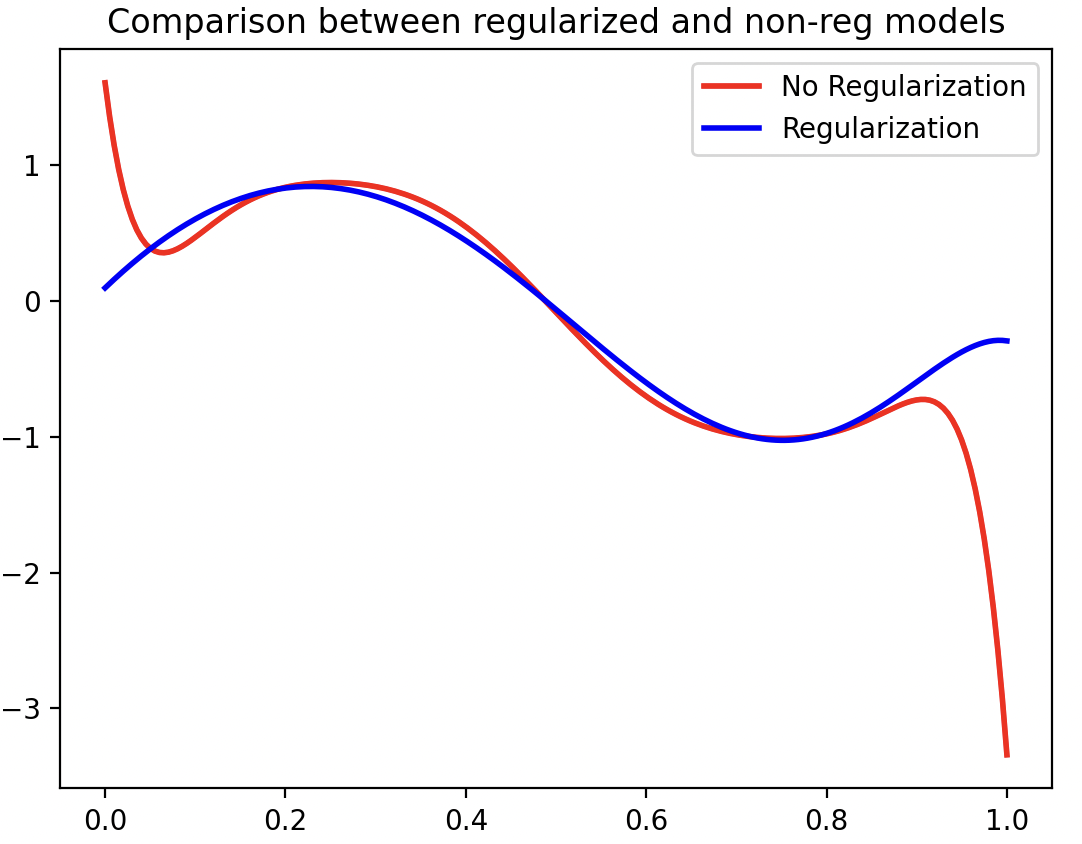
\includegraphics[width=0.5\linewidth]{3.3 Models.png}
    \caption{Enter Caption}
    \label{fig:enter-label}
\end{figure}

\subsection{Model Evaluation}
On the test set the MSE for the model with no regularization is 0.3565.  

The MSE for the model with regularization is 0.0335

\subsection{Large Set Regression}

\begin{figure}[H]
    \centering
    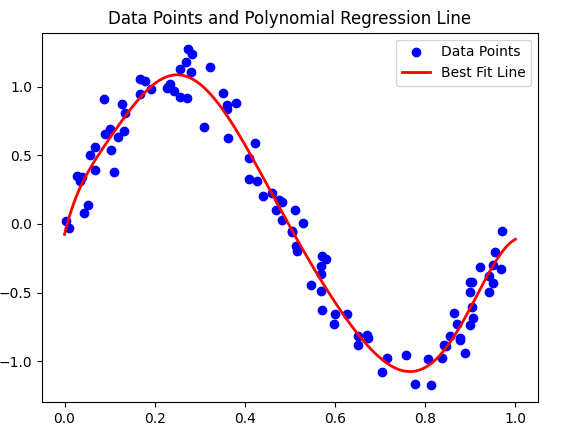
\includegraphics[width=0.5\linewidth]{3.5 LargeSet Regression Graph.png}
    \caption{Large Set Regression using n = 100}
\end{figure}

\subsection{Solutions to Control Complexity}
As seen in 3.3, using a regularization constant can control model complexity. The regularization constant penalizes large coefficients, thus reducing the chance of overfitting, especially with a polynomial of a high degree.

Also seen in 3.3, the use of cross-validation also can control model complexity. Cross-validation involves setting a side a portion of the training data to be used as a validation set. Training on each fold and testing on their respective validation set can show possible overfitting and underfitting. Taking the average of each of the models allows the model more generalizable.

Finally, in 3.5, we see that increasing the number of data points can also control model complexity. More data points decreases the effect that noise has on the generated model. It also reduces variance in the model, making the model less sensitive to small variations in the training data.

\newpage
\section{Eigenface}
\subsection{Spectral Decomposition}

See HW2Code- Q4

\subsection{Image Representation}

\begin{figure}[!htb]
   \begin{minipage}{0.48\textwidth}
     \centering
      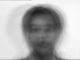
\includegraphics[width=0.5\linewidth]{pic0_M2.png}
    \caption{Subject 15: Centerlight M=2}
   \end{minipage}\hfill
   \begin{minipage}{0.48\textwidth}
     \centering
     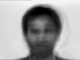
\includegraphics[width=.5\linewidth]{pic0_M10.png}
     \caption{Subject 15: Centerlight M=10}
   \end{minipage}
   \begin{minipage}{0.48\textwidth}
     \centering
     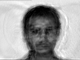
\includegraphics[width=.5\linewidth]{pic0_M100.png}
     \caption{Subject 15: Centerlight M=100}
   \end{minipage}
   \begin{minipage}{0.48\textwidth}
     \centering
     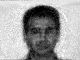
\includegraphics[width=.5\linewidth]{pic0_M1000.png}
     \caption{Subject 15: Centerlight M=1000}
   \end{minipage}
   \begin{minipage}{0.48\textwidth}
     \centering
     
\includegraphics[width=.5\linewidth]{pic0_M4000.png}
     \caption{Subject 15: Centerlight M=4000}
   \end{minipage}
\end{figure}

\subsection{Eigenvalues and Human Faces}

Displayed below are the eigenvectors that correspond to the 10 largest eigenvalues in the training set. In the pictures present we see that outlines and silhouettes of individual faces are seen, the general structure of the face and hair, and general facial features, albeit very blurry, like the nose, eyes, and mouth. The largest eigenvalue corresponds to the eigenvector that has the most variance throughout the dataset. As we move down the list, more specific but common features between the training faces are seen, such as in Eigenvector 8 with distinct facial detail.

\begin{figure}[!htb]
   \begin{minipage}{0.48\textwidth}
     \centering
      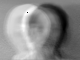
\includegraphics[width=0.5\linewidth]{eigenvector0.png}
    \caption{Eigenvector 0}
   \end{minipage}\hfill
   \begin{minipage}{0.48\textwidth}
     \centering
     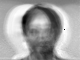
\includegraphics[width=.5\linewidth]{eigenvector1.png}
     \caption{Eigenvector 1}
   \end{minipage}
   \begin{minipage}{0.48\textwidth}
     \centering
     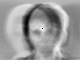
\includegraphics[width=.5\linewidth]{eigenvector2.png}
     \caption{Eigenvector 2}
   \end{minipage}
   \begin{minipage}{0.48\textwidth}
     \centering
     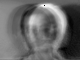
\includegraphics[width=.5\linewidth]{eigenvector3.png}
     \caption{Eigenvector 3}
   \end{minipage}
   \begin{minipage}{0.48\textwidth}
     \centering
     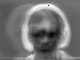
\includegraphics[width=.5\linewidth]{eigenvector4.png}
     \caption{Eigenvector 4}
   \end{minipage}
      \begin{minipage}{0.48\textwidth}
     \centering
     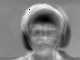
\includegraphics[width=.5\linewidth]{eigenvector5.png}
     \caption{Eigenvector 5}
   \end{minipage}
      \begin{minipage}{0.48\textwidth}
     \centering
     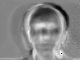
\includegraphics[width=.5\linewidth]{eigenvector6.png}
     \caption{Eigenvector 6}
   \end{minipage}
      \begin{minipage}{0.48\textwidth}
     \centering
     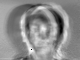
\includegraphics[width=.5\linewidth]{eigenvector7.png}
     \caption{Eigenvector 7}
   \end{minipage}
      \begin{minipage}{0.48\textwidth}
     \centering
     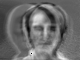
\includegraphics[width=.5\linewidth]{eigenvector8.png}
     \caption{Eigenvector 8}
   \end{minipage}
      \begin{minipage}{0.48\textwidth}
     \centering
     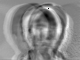
\includegraphics[width=.5\linewidth]{eigenvector9.png}
     \caption{Eigenvector 9}
   \end{minipage}
\end{figure}

\newpage
\section{Estimate Art Creation- Deep CNN}
\subsection{Pre-processing}
\begin{figure}[H]
    \centering
    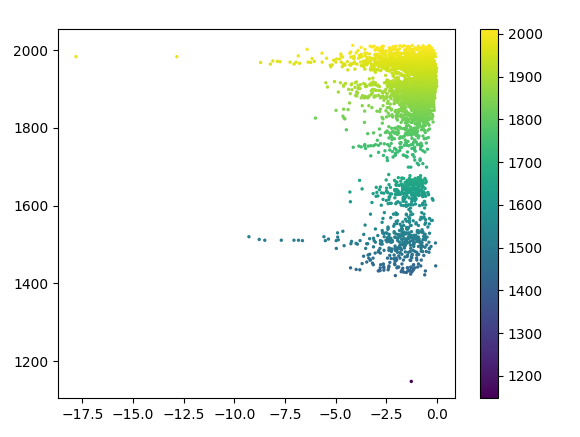
\includegraphics[width=0.5\linewidth]{5.1 2D Visualization.png}
    \caption{Year over m=1 PCA}
\end{figure}
\begin{figure}[H]
    \centering
    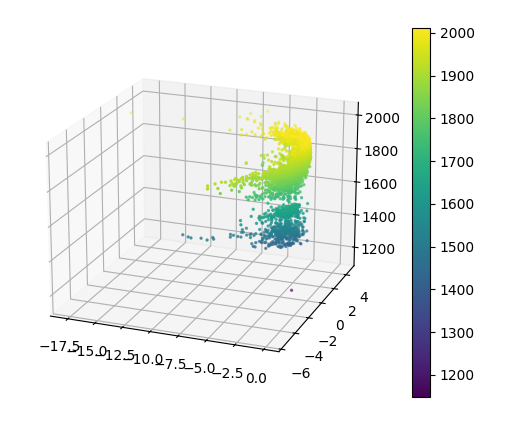
\includegraphics[width=0.5\linewidth]{5.1 3D Visualization.png}
    \caption{Year over m=2 PCA}
\end{figure}

Above are the plots for the data set with 1 and 2 principle components respectively. We see in the 3D (2-PC) that the 2D (1-PC) plot is insufficient in fully visualizing the variance in the data set. PCA aims to reduce dimensionality, while also retaining enough variance to draw meaningful inferences and models from the data set.

\subsection{Training}
\begin{figure}[H]
    \centering
    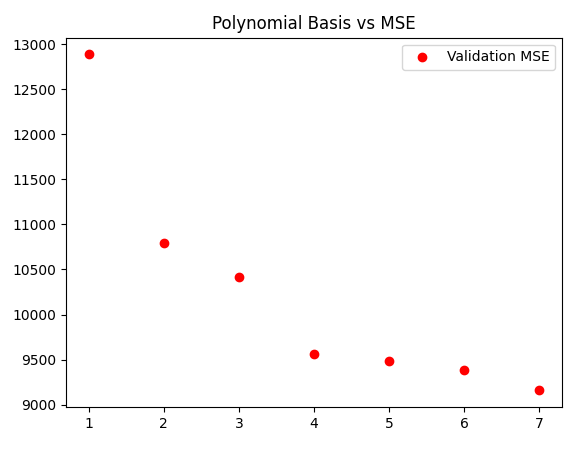
\includegraphics[width=0.5\linewidth]{5.2 Error.png}
\end{figure}


\subsection{Testing}

My Model MSE on the test set was 27888.523
My largest error was on "Christ before Herod" with a prediction of 2231, Actual: 1509 
My smallest error was on "Mikhail Ivanovich" with a prediction of 1893, Actual: 1893 
\end{document}